% Soubory musí být v kódování, které je nastaveno v příkazu \usepackage[...]{inputenc}

\documentclass[%        Základní nastavení
%  draft,    				  % Testovací překlad
  12pt,       				% Velikost základního písma je 12 bodů
  a4paper,    				% Formát papíru je A4
  %oneside,      			% Jednostranný tisk
	twoside,      			% Dvoustranný tisk (kapitoly a další důležité části tedy začínají na lichých stranách)
	unicode,						% Záložky a metainformace ve výsledném  PDF budou v kódování unicode
]{report}				    	% Dokument třídy 'zpráva', vhodná pro sazbu závěrečných prací s kapitolami

\usepackage[utf8]		  %	Kódování zdrojových souborů je UTF-8
	{inputenc}					% Balíček pro nastavení kódování zdrojových souborů

\usepackage[				  % Nastavení geometrie stránky
	bindingoffset=10mm,		% Hřbet pro vazbu
	hmargin={25mm,25mm},	% Vnitřní a vnější okraj  (jsou nehezky shodné; jakási úroveň estetiky je dosažena pomocí hřbetu)
	vmargin={25mm,34mm},	% Horní a dolní okraj
	footskip=17mm,			  % Velikost zápatí
	nohead,					      % Bez záhlaví
	marginparsep=2mm,		  % Vzdálenost marginálií
	marginparwidth=18mm,	% Šířka marginálií
]{geometry}

\usepackage{sectsty}
	%přetypuje nadpisy všech úrovní na bezpatkové, kromě \chapter, která je přenastavena zvlášť v thesis.sty
	\allsectionsfont{\sffamily}

\usepackage{graphicx} % Balíček 'graphicx' pro vkládání obrázků
											% Nutné pro vložení logotypů školy a fakulty

\usepackage[          % Balíček 'acronym' pro sazby zkratek a symbolů
	nohyperlinks				% Nebudou tvořeny hypertextové odkazy do seznamu zkratek
]{acronym}						
											% Nutné pro použití prostředí 'acronym' balíčku 'thesis'

\usepackage[
	breaklinks=true,		% Hypertextové odkazy mohou obsahovat zalomení řádku
	hypertexnames=false % Názvy hypertext. odkazů budou tvořeny nezávisle na názvech TeXu
]{hyperref}						% Balíček 'hyperref' pro sazbu hypertextových odkazů
											% Nutné pro použití příkazu 'pdfsettings' balíčku 'thesis'

\usepackage{pdfpages} % Balíček umožňující vkládat stránky z PDF souborů
                      % Nutné při vkládání titulních listů a zadání přímo
                      % ve formátu PDF z informačního systému

\usepackage{enumitem} % Balíček pro nastavení mezerování v odrážkách
  \setlist{topsep=0pt,partopsep=0pt,noitemsep} % konkrétní nastavení

\usepackage{cmap} 		% Balíček cmap zajišťuje, že PDF vytvořené `pdflatexem' je
											% plně "prohledávatelné" a "kopírovatelné"

%\usepackage{upgreek}	% Balíček pro sazbu stojatých řeckých písmem
											%% např. stojaté pí: \uppi
											%% např. stojaté mí: \upmu (použitelné třeba v mikrometrech)
											%% pozor, grafická nekompatibilita s fonty typu Computer Modern!
                      
%\usepackage{amsmath} %balíček pro sabu náročnější matematiky                 

\usepackage{dirtree}	% sazba adresářové struktury
                      % vhodné pro prezentaci obsahu elektronické přílohy (např. CD)

\usepackage[formats]{listings}	% Balíček pro sazbu zdrojových textů
\lstset{              % nastavení
%	Definice jazyka použitého ve výpisech
%    language=[LaTeX]{TeX},	% LaTeX
%	language={Matlab},		% Matlab
	language={C},           % jazyk C
    basicstyle=\ttfamily,	% definice základního stylu písma
    tabsize=2,			% definice velikosti tabulátoru
    inputencoding=utf8,         % pro soubory uložené v kódování UTF-8
		columns=fixed,  %fixed nebo flexible,
		fontadjust=true %licovani sloupcu
    extendedchars=true,
    literate=%  definice symbolů s diakritikou
    {á}{{\'a}}1
    {č}{{\v{c}}}1
    {ď}{{\v{d}}}1
    {é}{{\'e}}1
    {ě}{{\v{e}}}1
    {í}{{\'i}}1
    {ň}{{\v{n}}}1
    {ó}{{\'o}}1
    {ř}{{\v{r}}}1
    {š}{{\v{s}}}1
    {ť}{{\v{t}}}1
    {ú}{{\'u}}1
    {ů}{{\r{u}}}1
    {ý}{{\'y}}1
    {ž}{{\v{z}}}1
    {Á}{{\'A}}1
    {Č}{{\v{C}}}1
    {Ď}{{\v{D}}}1
    {É}{{\'E}}1
    {Ě}{{\v{E}}}1
    {Í}{{\'I}}1
    {Ň}{{\v{N}}}1
    {Ó}{{\'O}}1
    {Ř}{{\v{R}}}1
    {Š}{{\v{S}}}1
    {Ť}{{\v{T}}}1
    {Ú}{{\'U}}1
    {Ů}{{\r{U}}}1
    {Ý}{{\'Y}}1
    {Ž}{{\v{Z}}}1
}

%%%%%%%%%%%%%%%%%%%%%%%%%%%%%%%%%%%%%%%%%%%%%%%%%%%%%%%%%%%%%%%%%
%%%%%%      Definice informací o dokumentu             %%%%%%%%%%
%%%%%%%%%%%%%%%%%%%%%%%%%%%%%%%%%%%%%%%%%%%%%%%%%%%%%%%%%%%%%%%%%

% V tomto souboru se nastavují téměř veškeré informace, proměnné mezi studenty:
% jméno, název práce, pohlaví atd.
% Tento soubor je SDÍLENÝ mezi textem práce a prezentací k obhajobě -- netřeba něco nastavovat na dvou místech.

\usepackage[
%%% Z následujících voleb jazyka lze použít pouze jednu
  czech-english,		% originální jazyk je čeština, překlad je anglicky (výchozí)
  %english-czech,	  % originální jazyk je angličtina, překlad je česky
  %slovak-english,	% originální jazyk je slovenština, překlad je anglicky
  %english-slovak,	% originální jazyk je angličtina, překlad je slovensky
%
%%% Z následujících voleb typu práce lze použít pouze jednu
  semestral,		  % semestrální práce (výchozí)
  %bachelor,			%	bakalářská práce
  %master,			  % diplomová práce
  %treatise,			% pojednání o disertační práci
  %doctoral,			% disertační práce
%
%%% Z následujících voleb zarovnání objektů lze použít pouze jednu
%  left,				  % rovnice a popisky plovoucích objektů budou zarovnány vlevo
	center,			    % rovnice a popisky plovoucích objektů budou zarovnány na střed (vychozi)
%
]{thesis}   % Balíček pro sazbu studentských prací


%%% Jméno a příjmení autora ve tvaru
%  [tituly před jménem]{Křestní}{Příjmení}[tituly za jménem]
% Pokud osoba nemá titul před/za jménem, smažte celý řetězec '[...]'
\author[]{Tomáš}{Vavrinec}

%%% Identifikační číslo autora (VUT ID)
\butid{240893}

%%% Pohlaví autora/autorky
% (nepoužije se ve variantě english-czech ani english-slovak)
% Číselná hodnota: 1...žena, 0...muž
\gender{0}

%%% Jméno a příjmení vedoucího/školitele včetně titulů
%  [tituly před jménem]{Křestní}{Příjmení}[tituly za jménem]
% Pokud osoba nemá titul před/za jménem, smažte celý řetězec '[...]'
\advisor[doc.\ Ing..]{Pavel}{Šteffan}[Ph.D.]

%%% Jméno a příjmení oponenta včetně titulů
%  [tituly před jménem]{Křestní}{Příjmení}[tituly za jménem]
% Pokud osoba nemá titul před/za jménem, smažte celý řetězec '[...]'
% Nastavení oponenta se uplatní pouze v prezentaci k obhajobě;
% v případě, že nechcete, aby se na titulním snímku prezentace zobrazoval oponent, pouze příkaz zakomentujte;
% u obhajoby semestrální práce se oponent nezobrazuje (jelikož neexistuje)
% U dizertační práce jsou typicky dva až tři oponenti. Pokud je chcete mít na titulním slajdu, prosím ručně odkomentujte a upravte jejich jména v definici "VUT title page" v souboru thesis.sty.
\opponent[doc.\ Mgr.]{Křestní}{Příjmení}[Ph.D.]

%%% Název práce
%  Parametr ve složených závorkách {} je název v originálním jazyce,
%  parametr v hranatých závorkách [] je překlad (podle toho jaký je originální jazyk).
%  V případě, že název Vaší práce je dlouhý a nevleze se celý do zápatí prezentace, použijte příkaz
%  \def\insertshorttitle{Zkác.\ náz.\ práce}
%  kde jako parametr vyplníte zkrácený název. Pokud nechcete zkracovat název, budete muset předefinovat,
%  jak se vytváří patička slidu. Viz odkaz: https://bit.ly/3EJTp5A
\title[Title of Student's Thesis]{Automatické herní stanoviště}

%%% Označení oboru studia
%  Parametr ve složených závorkách {} je název oboru v originálním jazyce,
%  parametr v hranatých závorkách [] je překlad
\specialization[Microelectronics and Technology]{Mikroelektronika a technologie}

%%% Označení ústavu
%  Parametr ve složených závorkách {} je název ústavu v originálním jazyce,
%  parametr v hranatých závorkách [] je překlad
%\department[Department of Control and Instrumentation]{Ústav automatizace a měřicí techniky}
%\department[Department of Biomedical Engineering]{Ústav biomedicínského inženýrství}
%\department[Department of Electrical Power Engineering]{Ústav elektroenergetiky}
%\department[Department of Electrical and Electronic Technology]{Ústav elektrotechnologie}
%\department[Department of Physics]{Ústav fyziky}
%\department[Department of Foreign Languages]{Ústav jazyků}
%\department[Department of Mathematics]{Ústav matematiky}
\department[Department of Microelectronics]{Ústav mikroelektroniky}
%\department[Department of Radio Electronics]{Ústav radioelektroniky}
%\department[Department of Theoretical and Experimental Electrical Engineering]{Ústav teoretické a experimentální elektrotechniky}
% \department[Department of Telecommunications]{Ústav telekomunikací}
%\department[Department of Power Electrical and Electronic Engineering]{Ústav výkonové elektrotechniky a elektroniky}

%%% Označení fakulty
%  Parametr ve složených závorkách {} je název fakulty v originálním jazyce,
%  parametr v hranatých závorkách [] je překlad
%\faculty[Faculty of Architecture]{Fakulta architektury}
\faculty[Faculty of Electrical Engineering and~Communication]{Fakulta elektrotechniky a~komunikačních technologií}
%\faculty[Faculty of Chemistry]{Fakulta chemická}
%\faculty[Faculty of Information Technology]{Fakulta informačních technologií}
%\faculty[Faculty of Business and Management]{Fakulta podnikatelská}
%\faculty[Faculty of Civil Engineering]{Fakulta stavební}
%\faculty[Faculty of Mechanical Engineering]{Fakulta strojního inženýrství}
%\faculty[Faculty of Fine Arts]{Fakulta výtvarných umění}
%
%Nastavení logotypu (v hranatych zavorkach zkracene logo, ve slozenych plne):
\facultylogo[logo/FEKT_zkratka_barevne_PANTONE_CZ]{logo/UTKO_color_PANTONE_CZ}

%%% Rok odevzdání práce
\graduateyear{2023}
%%% Akademický rok odevzdání práce
\academicyear{2023/24}

%%% Datum obhajoby (uplatní se pouze v prezentaci k obhajobě)
\date{11.\,11.\,1980} 

%%% Místo obhajoby
% Na titulních stránkách bude automaticky vysázeno VELKÝMI písmeny (pokud tyto stránky sází šablona)
\city{Brno}

%%% Abstrakt
\abstract[%
The aim of this thesis is to design an electronic device for use in outdoor games. 
Primarily the design of an automatic gaming station, but there has also been a design of a simple personal device. 
This thesis deals with the selection and rough design of the electronics.
Emphasis is placed on the selection of appropriate systems for application in games and the design of electronics based on these.
The design is divided into several groupings, the personal device design and the game station design which is further divided into the design of the core and its modules.
]{%
Cílem práce je navrhnout elektronické zařízení pro využití v outdorových hrách. 
Primárně jde o návrh automatického herního stanoviště, ale došlo i k návrhu jednoduchého osobního zařízení. 
Tato práce se zabývá teoretickým návrhem elektroniky.
Je kladen důraz na výběr vhodných systémů k aplikaci ve hrách a z nich vychází návrh elektroniky.
Návrh je rozdělen do několika skupin, návrh osobního zařízení a návrh herního stanoviště, který se dále dělí na návrh jádra a jeho modulů.
}

%%% Klíčová slova
\keywrds[%
microcontroller, ESP32, ESP32-C3-MINI-1, ESP32-S3, ESP32-S3-WROOM, outdoor games, gaming stations, gaming facilities
]{%
mikrokontrolér, ESP32, ESP32-C3-MINI-1, ESP32-S3, ESP32-S3-WROOM, outdoorové hry, herní stanoviště, herní zařízení
% Klíčová slova v~originálním jazyce
}

%%% Poděkování
\acknowledgement{%
Rád bych poděkoval vedoucímu semestrální práce
panu doc. Ing. Pavlu Šteffanovi, Ph.D.\ za odborné vedení,
konzultace, trpělivost a~podnětné návrhy k~práci.
}%  % do tohoto souboru doplňte údaje o sobě, druhu práce, názvu...

%%%%%%%%%%%%%%%%%%%%%%%%%%%%%%%%%%%%%%%%%%%%%%%%%%%%%%%%%%%%%%%%%%%%%%%%

%%%%%%%%%%%%%%%%%%%%%%%%%%%%%%%%%%%%%%%%%%%%%%%%%%%%%%%%%%%%%%%%%%%%%%%%
%%%%%%     Nastavení polí ve Vlastnostech dokumentu PDF      %%%%%%%%%%%
%%%%%%%%%%%%%%%%%%%%%%%%%%%%%%%%%%%%%%%%%%%%%%%%%%%%%%%%%%%%%%%%%%%%%%%%
%% Při načteném balíčku 'hyperref' lze použít příkaz '\pdfsettings':
\pdfsettings
%  Nastavení polí je možné provést také ručně příkazem:
%\hypersetup{
%  pdftitle={Název studentské práce},    	% Pole 'Document Title'
%  pdfauthor={Autor studenstké práce},   	% Pole 'Author'
%  pdfsubject={Typ práce}, 						  	% Pole 'Subject'
%  pdfkeywords={Klíčová slova}           	% Pole 'Keywords'
%}
%%%%%%%%%%%%%%%%%%%%%%%%%%%%%%%%%%%%%%%%%%%%%%%%%%%%%%%%%%%%%%%%%%%%%%%

\pdfmapfile{=vafle.map}

%%%%%%%%%%%%%%%%%%%%%%%%%%%%%%%%%%%%%%%%%%%%%%%%%%%%%%%%%%%%%%%%%%%%%%%
%%%%%%%%%%%       Začátek dokumentu               %%%%%%%%%%%%%%%%%%%%%
%%%%%%%%%%%%%%%%%%%%%%%%%%%%%%%%%%%%%%%%%%%%%%%%%%%%%%%%%%%%%%%%%%%%%%%
\begin{document}
\pagestyle{empty} %vypnutí číslování stránek

%%% Vložení desek -- od září 2021 na žádost fakulty nepoužíváno
%\includepdf[pages=1]%  buďto generovaných informačním systémem
  %{pdf/student-desky}% název souboru nesmí obsahovat mezery!
%%% NEBO vytvoření desek z balíčku
%%\makecover
%%%
%\oddpage % při dvojstranném tisku přidá prázdnou stránku
%% kazdopádně ale:
%\setcounter{page}{1} %resetovaní čítače stránek -- desky do číslování nezahrnujeme

%% Vložení titulního listu
\includepdf[pages=1]%    buďto generovaného informačním systémem
  {pdf/student-titulka}% název souboru nesmí obsahovat mezery!
%% NEBO vytvoření titulní stránky z balíčku
%\maketitle
%%
\oddpage  % při dvojstranném tisku se přidá prázdná stránka
   
%% Vložení zadání
\includepdf[pages=1]%   buďto generovaného informačním systémem
  {pdf/student-zadani}% název souboru nesmí obsahovat mezery!
%% NEBO lze vytvořit prázdný list příkazem ze šablony
%\patternpage{}%
%	{\sffamily\Huge\centering ZDE VLOŽIT LIST ZADÁNÍ}%
%	{\sffamily\centering Z~důvodu správného číslování stránek}
%%
\oddpage% při dvojstranném tisku se přidá prázdná stránka

%% Vysázení stránky s abstraktem
\makeabstract

% Vysázení stránky s rozšířeným abstraktem
% (pokud píšete práci v češtině či slovenštině, vložení rozšířeného abstraktu zrušte;
%  pro semestrální projekt také není potřeba rozšířený abstrakt uvádět)
% Vysázení stránky s rozšířeným abstraktem
% (týká se pouze bc. a dp. prací psaných v angličtině, viz Směrnice rektora 72/2017)
\cleardoublepage
\noindent
{\large\sffamily\bfseries\MakeUppercase{Rozšířený abstrakt}}
\\
Výtah ze směrnice rektora 72/2017:\\
\emph{Bakalářská a diplomová práce předložená v angličtině musí obsahovat rozšířený abstrakt v češtině
nebo slovenštině (čl. 15). To se netýká studentů, kteří studují studijní program akreditovaný v
angličtině.}
(čl. 3, par. 7)\\
\emph{Nebude-li vnitřní normou stanoveno jinak, doporučuje se rozšířený abstrakt o rozsahu přibližně 3
normostrany, který bude obsahovat úvod, popis řešení a shrnutí a~zhodnocení výsledků.}
(čl. 15, par. 5)

%%% Vysázení citace práce
\makecitation

%%% Vysázení prohlášení o samostatnosti
\makedeclaration

%%% Vysázení poděkování
\makeacknowledgement

%%% Vysázení obsahu
\tableofcontents

%%% Vysázení seznamu obrázků
% (vynechejte, pokud máte dva nebo méně obrázků)
\listoffigures

%%% Vysázení seznamu tabulek
% (vynechejte, pokud máte dvě nebo méně tabulek)
\listoftables

%%% Vysázení seznamu výpisů kódu
% (vynechejte, pokud máte dva nebo méně výpisů)
\lstlistoflistings

\cleardoublepage\pagestyle{plain}   % zapnutí číslování stránek

%Pro vkládání kapitol i příloh používejte raději \include než \input
%%% Vložení souboru 'text/uvod.tex' s úvodem

\chapter*{Úvod}
%Automatické herní stanoviště (AHS) je nástroj pro tvorbu outdoorových her.
Outdoorové hry bývají často složeny ze stanovišť, na kterých mají hráči plnit různé úkoly.
Aby bylo možné tyto úkoly zadat a vyhodnotit jejich výsledek, je většinou nutné, aby na stanovišti byl nějaký organizátor a stanoviště obsluhoval.
Tyto úkoly jsou ale často poměrně prosté a není tak problém je automatizovat, což může organizátory uvolnit k jiné činnosti.
Outdoorové hry by navíc znatelně oživila aktivní komunikace mezi stanovištěmi, která by tak mohla i vytvořit prostor pro nové herní mechaniky.

Řada outdoorových her využívá různé podomácku vyrobené zařízení, které nějaký z organizátorů postavil za účelem konkrétní hry.
Taková zařízení ale autora stojí velké množství času, protože jej musí celé od základu navrhnout, vyrobit a navíc je jej pak schopen obsluhovat jen on.
Navíc je pak takové zařízení typicky použito jen u jedné nebo dvou her, po kterých jej autor buď, rozebere, nebo bezpečně uloží někam, kde si jej náhodou všimne o deset let později při úklidu.
V neposlední řadě bývají jakýmsi zlatým hřebem celé akce např. týdenního tábora a jejich kouzlo je především v odlišnosti od zbytku akce.



Z těchto důvodů padlo rozhodnutí na vývoj univerzálního automatického herního stanoviště, které by se dalo opakovaně použít na různé hry i ve větší počtu.
Podstatnou součástí je pochopitelně i pokud možno co nejintuitivnější ovládání, aby uživatele nezdržovalo od zábavy.


% % Úvod studentské práce, např\,\dots

% % Nečíslovaná kapitola Úvod obsahuje \uv{seznámení} čtenáře s~problematikou práce.
% % Typicky se zde uvádí:
% % (a) do jaké tematické oblasti práce spadá, (b) co jsou hlavní cíle celé práce a (c) jakým způsobem jich bylo dosaženo.
% % Úvod zpravidla nepřesahuje jednu stranu.
% % Poslední odstavec Úvodu standardně představuje základní strukturu celého dokumentu.

% % Tato práce se věnuje oblasti \acs{DSP} (\acl{DSP}), zejména jevům, které nastanou při nedodržení Nyquistovy podmínky pro \ac{symfvz}.%
% % \footnote{Tato věta je pouze ukázkou použití příkazů pro sazbu zkratek.}

% % Šablona je nastavena na \emph{dvoustranný tisk}.
% % Nebuďte překvapeni, že ve vzniklém PDF jsou volné stránky.
% % Je to proto, aby důležité stránky jako např.\ začátky kapitol začínaly po vytisknutí a svázání vždy na pravé straně.
% % %
% % Pokud máte nějaký závažný důvod sázet (a~zejména tisknout) jednostranně, nezapomeňte si přepnout volbu \texttt{twoside} na \texttt{oneside}!

% %%% Vložení souboru 'text/cile.tex' s úvodem
% \chapter*{Cíle práce}
\phantomsection
\addcontentsline{toc}{chapter}{Cíle práce}

Konkrétní specifikace cílů, které má autor v~práci vyřešit.
Tato kapitola je \emph{volitelná} -- pokud váš studijní program nevyžaduje zvláštní kapitolu s cíli,
cíle specifikujte v~rámci Úvodu.

%%% Vložení souboru 'text/reseni' s popisem řešení práce
% (rozdělte na více souborů či kapitol, pokud je vhodné)
\chapter{Teoretická část}
\section{Potřeby herních zařízení}
Outdoorové hry často mají nějaký příběh, který se dá vyprávět konkrétními úkoly na stanovištích.
Na některých stanovištích proto musí být lidská obsluha, na jiných ale může být lidská obsluha z příběhového pohledu nežádoucí.
Když má hráč například vyřadit automatický bezpečnostní systém je lidská obsluha stanoviště poslední možnost.
Podobná stanoviště proto bývají realizovány pomocí různých papírků a provázků.
To určitě má své kouzlo, ale i tak je u podobného stanoviště vhodné mít obsluhu.
Elektronické řešení podobných stanovišť by ale mohlo otevřít úplně nový svět možností.

%% Položme si tedy otázku, jak by takové zařízení mohlo vypadat.
Podstatný fakt je, že prakticky všichni u sebe dnes mají chytrý telefon, čehož můžeme využít.
Nemá proto velký význam, aby toto zařízení suplovalo funkce telefonu.
Např. grafický výstup typu display proto v podobném zařízení není potřeba, a v tomto směru už odvádí telefon naprosto dostatečnou práci.
Pokud by tedy v rámci hry bylo potřeba například předat hráči nějaký text nebo obrázek, může jej zařízení poslat uživateli na telefon.
Možnost propojení s telefonem je také velmi významná při nastavování hry.
Díky telefonu totiž zařízení nepotřebuje uživatelské rozhraní přizpůsobené nastavování.

Mohlo by se zdát, že herní stanoviště vlastně ani není potřeba a stačila by mobilní aplikace.
Ale přestože je mobil ve hrách dobře využitelný, jsou aplikace, na které jednoduše vhodný není.
Pokud má hráč například ze stanoviště získat nějaký fyzický objekt, mobil neposlouží.
Pro hráče ani organizátory také nemusí být zrovna komfortní před hrou zařizovat, aby měli všichni nainstalovaný správný software.
% Telefon také není například na stanovišti v lese dobře viditelný.
V neposlední řadě jde také o jistý "cool efekt", který běžné zařízení jako mobil nebo třeba tablet neposkytne. %%TODO: tohle chce nějak přeformulovat

Zařízení určené primárně pro outdoorové hry bychom mohli rozdělit na dvě skupiny, statické a dynamické, protože jsou na tyto skupiny kladeny výrazně jiné požadavky.
Dynamická zařízení jsou ta, která může uživatel pohodlně nosit s sebou.
Do dynamických zařízení by se tak dal zařadit právě i telefon, ten však může být z různých důvodu nevhodný a proto i tato zařízení dává smysl navrhnout specificky pro hry.
Statické zařízení je naopak zařízení, u kterého se nepředpokládá, že jej bude hráč nosit s sebou.
Přesto by mělo být jednoduše přenositelné, má jít o stanoviště, které se jednoduše donese na své místo a během hry se s ním nebude pohybovat.
Takové zařízení by tedy mělo být dobře viditelné a splňovat požadavky, které na něj konkrétní hra klade. %%TODO: tohle chce nějak přeformulovat?
Požadavky různých her můžou být ale dost rozdílné, častým požadavkem je něco uchovávat a např. po zadání hesla hráči vydat.
Hra ale taky může vyžadovat, aby bylo zařízení sto přehrát nějakou audio nahrávku nebo naopak pořídit záznam. %%TODO: tohle chce nějak přeformulovat?
Z těchto důvodů považujeme za vhodnější zařízení koncipovat jako základní řídící jednotku, která je samostatně funkční a použitelná při hře, ale ke které se dají jednoduše připojit moduly pro konkrétní herní mechaniky.

\section{Základní řídící jednotka}
% Z toho plyne otázka, jaká funkcionalita je potřebná v základním zařízení?
Asi žádný systém, se kterým hráč přímo interaguje, není nutný v každé hře.
Jde tedy o to vybrat takové systémy, které svými nároky nepřevýší užitečnost při hrách.
Ze zkušeností považujeme za nejzákladnější systém nějaký světelný výstup, ten dokáže většinu her velmi příjemně ozvláštnit.
Většinou je nezbytný i nějaký uživatelský vstup, na což většinou stačí obyčejná tlačítka.
Problém je ale určit jaké a kolik jich bude potřeba.
Některé hry vyžadují třeba jen jedno, ale takové, aby se do něj dalo co nejpohodlněji praštit v běhu, protože je zrovna cílem ke stanovišti co nejrychleji doběhnout.
Jiná hra může vyžadovat tlačítek víc, ale už není potřeba, aby byly tak velké, protože hráč při jejich používání nebude tak akční, ale bude třeba zadávat výsledek nějakého logického úkolu.
Univerzálnější je tedy nepoužívat tlačítka, ale nějaký systém, který se dá softwarově přizpůsobit.
Příkladem může být dotyková plocha, která se dá softwarově rozdělit na různé oblasti sloužící jako tlačítka a i během hry se tak dá počet tlačítek měnit.
Další důležitou vlastností je možnost komunikace s ostatními zařízeními, která do hry přináší novou možnost jak stanoviště propojit a také pohodlnou metodu jak stanoviště nastavit přes telefon.
V neposlední řade je potřeba nějaký zvukový výstup, který může být použit např. jako potvrzení zadaného hesla.

Z toho nám tedy plyne diagram \ref{fig:diagram_zanoreni_0}.
\begin{figure}[h]
    \centering
    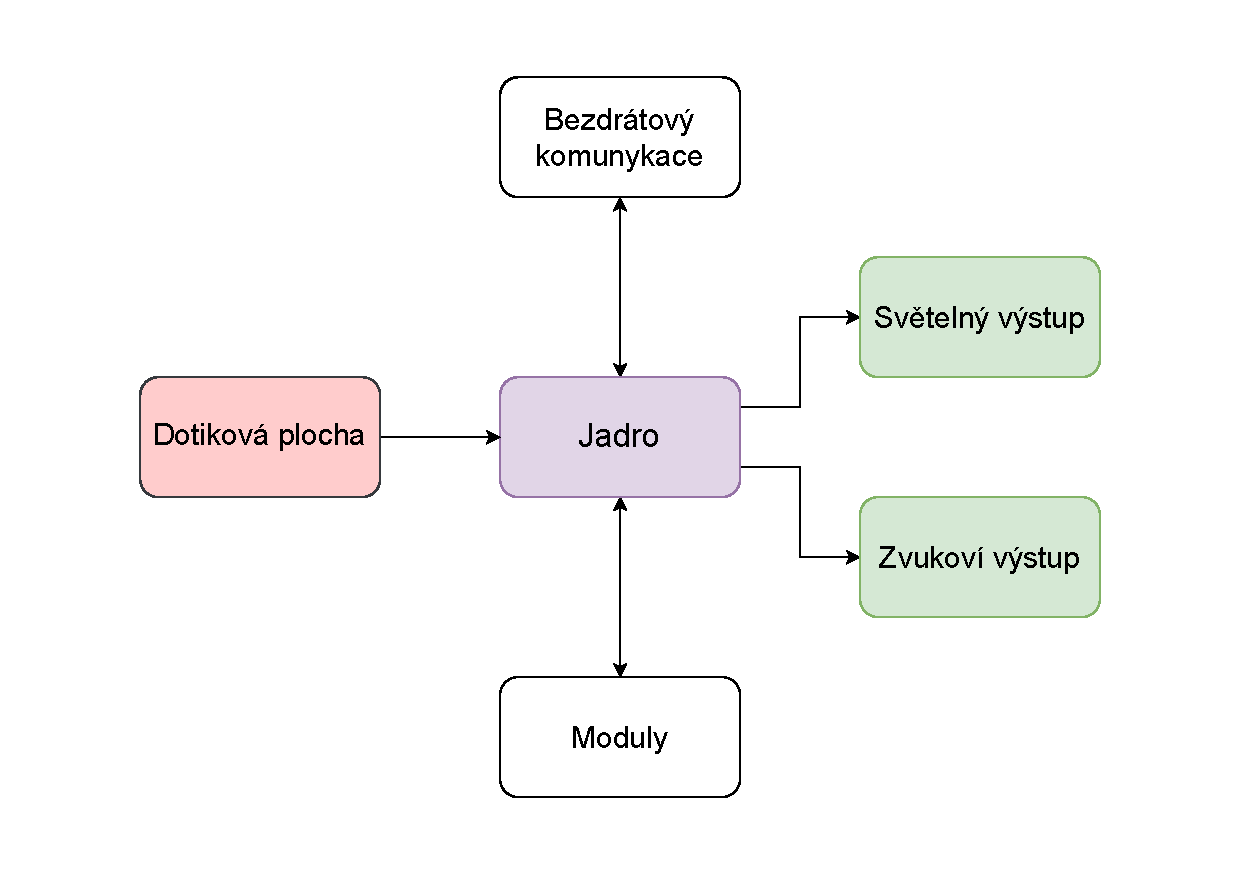
\includegraphics[width=0.65\textwidth]{text/TeoretickyUvod/AplikaceHernichZarizeni/diagram/zanoreni_0.pdf}
    \caption{Úvodní blokové schéma zařízení}
    \label{fig:diagram_zanoreni_0}
\end{figure}

\newpage

Co se světelného výstupu týče, na signalizaci různých stavů je vhodné používat různé barvy světel.
% Jaký vzhled by ale měl mít zdroj barevného světla na podobném zařízení?
Jak je uvedeno výše, není potřebné suplovat grafický display, za tímto účelem se dá použít propojení s telefonem.
Informace, kterou by zařízením mohlo často poskytovat je čas a směr, např. čas do konce kola nebo směr k dalšímu úkolu.
Podobné informace se dají elegantně zobrazit na kruhu.
Protože má být stanoviště viditelné i z větší vzdálenosti, je tedy otázkou, zda použít jen jeden kruh, tak aby byl dostatečně viditelný, nebo jich použít více. %%TODO: otázka co s totu otázkou?
Zobrazování pracuje ve dvou režimech, čtení na dálku a čtení na blízko.
Pro čtení na blízko je cílem přímá interakce se zařízením např. už zmiňované zadávání hesla.
Čtení na dálku je naopak určeno pro předávání informací hráči, když právě přímo neinteraguje se stanovištěm, např. který tým má zrovna povolený přístup.
Proto je vhodné mít kruhů víz, aby bylo možné zobrazovat tyto informace na různých kruzích, které mohou navíc být svému účelu přizpůsobeny.
Jeden kruh tak může svítit jen jedním směrem aby ho hráč vyděl celí najednou pro blízkou interakci, zatímco druhý kruh může svítit do všech stran aby byl vidět z co nejvíce míst.

Potřeba propojení s telefonem nám omezuje možnosti co se týče bezdrátové komunikace, protože telefony jsou většinou vybavený Bluetooth a WiFi.
Také se v telefonech rozšiřuje NFC, to je však pro tuto aplikaci z duvodu krátkého dosahu nevhodné.

Posledním systémem který je potřeba je zvukový výstup.
Protože většinou stačí jen jednoduchá zvuková odezva, není potřeba plnohodnotný zvukový systém.
Pro hry, které budou potřebovat přehrávat nějakou nahrávku bude samostatný zvukový modul, případně je možnost nahrávku přehrát přes uživatelův telefon.
V základním zařízení je proto potřeba jen jednoduchý bzučák, například jako odezva na kliknutí.

Můžeme tedy diagram upravit na \ref{fig:diagram_zanoreni_1}.
\begin{figure}[h]
    \centering
    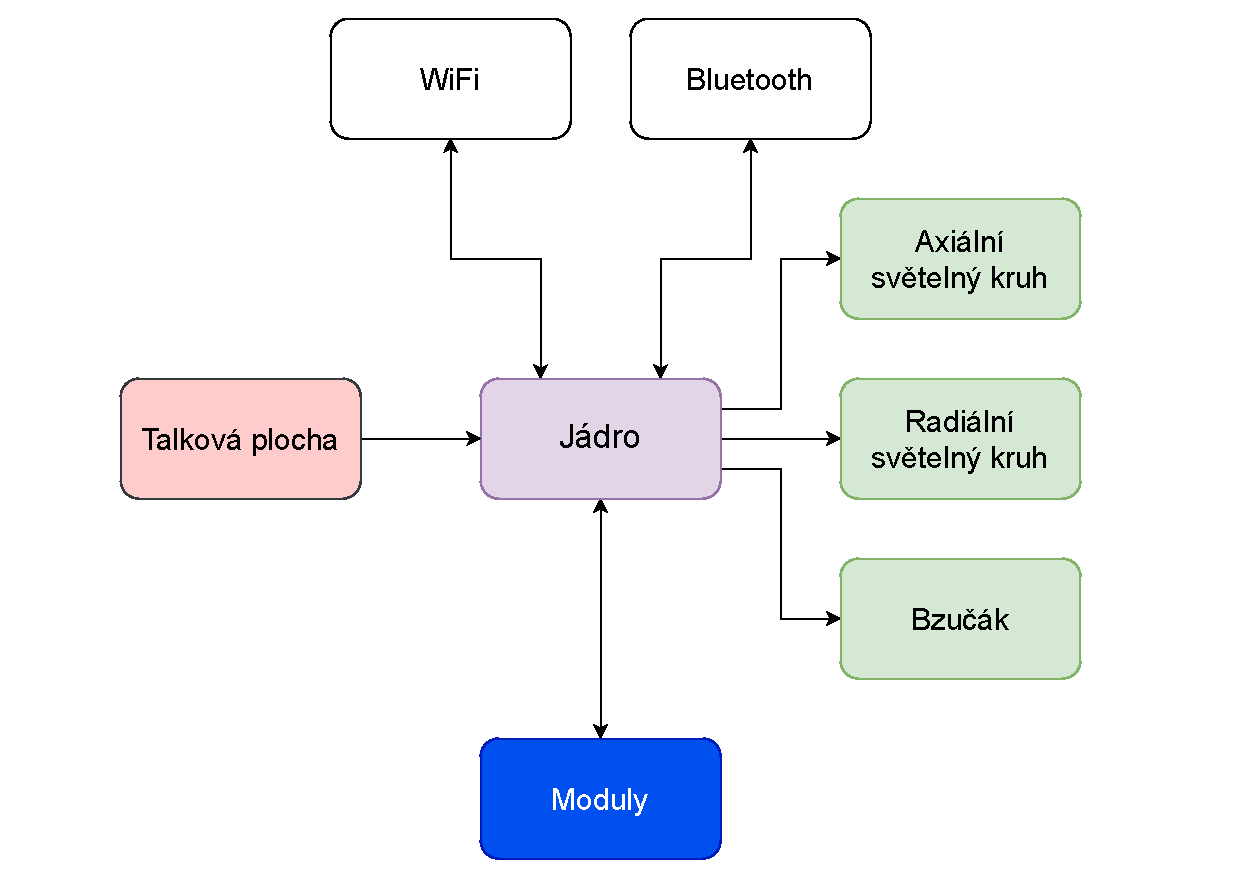
\includegraphics[width=0.65\textwidth]{text/TeoretickyUvod/AplikaceHernichZarizeni/diagram/zanoreni_1.pdf}
    \caption{Základního blokové schéma zařízení}
    \label{fig:diagram_zanoreni_1}
\end{figure}

\vspace{-10mm}
\section{Moduly}
Základní řídící jednotka je tedy schopná poskytnout základní funkce, které jsou potřeba pro většinu her.
Některé hry ale mohou vyžadovat nějakou specifickou funkci, kterou základní zařízení nedokáže poskytnout.
Proto je vhodné, aby bylo možné k základnímu zařízení připojit externí moduly, bez kterých by se konkrétní hry neobešli.

Jedním z takových modulů může být například modul dvířka, který umožní do zařízení uložit nějaký objekt a vydat jej jen po nějaké interakci.
Konkrétně má takový modul několik samostatných zamykatelných přihrádek, které se dají samostatně ovládat a mohou sloužit např. pro více týmů nebo uchovávat více objektu do různých částí hry.

Jednoduchá hrou která vyžaduje modul dvířka je např. hra Maják. %%TODO: vymyslet lepčí název tohle se  mi moc nepozdává (je to název z her od Petra na první lucerný v roce 2021)
V této hře jsou hráči rozděleni do týmů a každý tým má svou barvu, od které je odvozena konkrétní přihrádka. 
Týmy mají za úkol získat co nejvíc sad kartiček.
Na hřišti je několik automatických stanovišť s modulem dvířka a v každém z nich je nějaký typ kartičky.
Každé stanoviště během hry umožňuje přístup právě jednomu týmu, které v pravidelném intervalu mění a čas do změny reprezentuje na jednom z kruhů.
Při startu hry si každé stanoviště náhodně vybere tým kterým začne a následně se už drží konstantního pořadí.
Když někdo dorazí ke stanovišti ve chvíli kdy má stanoviště zpřístupnění jeho tým a klepne na tlakovou plochu, stanoviště mu vydá kartičku.
Stanoviště se týmu zpřístupní jen v čase daného týmu a navíc jen jednou za kolo.
Hráčům cíleně není představen celí mechanizmus výdeje kartiček, je jim řečeno jen že se přihrádka otevírá klepnutím do tlakové plochy a že je zajímají jen kartičky jejich barvi. 
Tým tedy musí spolupracovat nejprve na odhalení mechanizmu a následně myslet jak tedy zvítězit.

Podobná hra se duď dá hrát samostatně nebo muže jít například jen o metodu jak získávat suroviny v nějaké komplexnější hře.

Další modul, který se dá připojit je zvukový modul.
Hra který vyžaduje zvukový modul je například hra s názvem Ticho.
Tato hrá vyžaduje zároveň i modul dvířka.
V této hře stanoviště sleduje intenzitu zvuku v okoli a v momente kdy hluk klesne pod stanovenou úroveň stanoviště otevře dvířka. 
% Ucastnikum není ovládání představeno a musí tak na něj přijít samy.
Stanoviště je hráčům představeno jako "magicka krabicka" za carou ke ktere se nesmi proplížit ale muzou ji z dalky ovlivnit.
Ukolem hracu tak bylo prijit na to jak lucerna funguje a jak ji presvedci aby se otevřela.

V rámci zvukového modulu je i možnost přehrát nějakou nahrávku.
Tato část zvukového modulu umožňuje intenzivnější vtažení hráče do hry s příběhem.
Může jít například o unikovou hru při které hráč ocitne v oblasti v neznámém bludišti a jeho úkolem je najít cestu ven.
Při hledání muže narazit na různá stanoviště která mu nejprve přehrají nějakou část příběhu a následně mu dají nějaký úkol nebo radu jak postupovat dál.

Podstatným modulem je také komunikační modul který umožňuje připojení k mobilní síti a tím i komunikaci s ostatními zařízeními na velkou vzdálenost.
Tento modul je potřeba například pro hru Zábor kopce.

V této hře se na hřišti o velké rozloze nachází několik automatických stanovišť.
Hráči jsou rozděleni do týmů a každý tým má svou barvu a své tlačítko na stanovišti označené barvou týmu.
V hře Zábor Kopce je hlavním cílem získávat body pro svůj tým ovládnutím a udržením stanovišť na rozsáhlém hřišti. 
Axiálním světelný kruh zobrazuje rozdělení tlakové plochu na jednotlivá tlačítka týmů podle jejich barvi.
Zabrání stanoviště pak mohou hráči provést stiskem příslušného tlačítka. 
Získávání bodů se odehrává dvěma způsoby, ovládnutím stanoviště a následným držením stanoviště pod kontrolou. 
Týmy mohou přebírat stanoviště od soupeřů, což přidává hře strategický rozměr. 
Výhodou je kontrolovat více stanovišť najednou, což umožňuje rychlejší získávání bodů a zvyšuje šanci na vítězství.
Komunikační modul je tu potřebný pro vyhodnocování hry.
Stanoviště totiž musí být schopné komunikovat s centrálním serverem, který vyhodnocuje hru a zobrazuje její průběh.
Tato hra je původně navržena pro airsoftové hráče na hřiště v Mokra-Horakov o rozloze \(6.7\-[ha]\) \cite{MokraHorakov}.
V takovém prostředí je tedy komunikace pomocí WiFi či Bluetooth nedostačuje, protože stanoviště mohou být i několik set metrů od sebe.

\subsection{Výběr bezdrátové komunikace dlouhého dosahu}
Pro komunikaci na dlouhé vzdálenosti se nabízí asi jen dvě základní možnosti, LoRa a mobilní síť.
Ještě počátkem roku 2023 by byla i třetí možnost, Sigfox, ale jeho síť byla v ČR vypnuta \cite{SigfoxKonci}.

LoRa je technologie určená pro komunikaci na dlouhé vzdálenosti s malou spotřebou a datovou propustností.
Pracuje v bezlicenčním pásmu a není tedy třeba platit za provoz.
Její dosah je i v zastavěné oblasti v řádu kilometru \cite{LoRaSEMTECH}, a za ideálních podmínek na přímou viditelnost i přes sto kilometru \cite{LoRaEMAN}. 
Nevýhoda LoRy je ale malá datová propustnost ještě snížená omezením času provozu na \(1\-\%\)\cite{LoRaEMAN}.

Mobilní síď má v porovnání s LoRou výrazně větší datovou propustnost, ale na druhou stranu je třeba platit za provoz a je méně energeticky úsporná.
Například NB-IoT je energeticky asi o třetinu náročnější než LoRa.
Přesto je dostatečně úsporná aby bylo zařízení, které tuto technologii využívá, sto běžet na baterii přes deset let \cite{LoRaVSNB-IoT}.
Energetická náročnost tedy není problém a vyšší datová propustnost společně s připojením na internet je významnější výhoda než bezplatný provoz u LoRy.
Další výhodou LoRy by mohla být nezávislost na pokrytí mobilní sítí, ale vzhledem k tomu, že pokrytí NB-IoT sítě je v ČR údajně \(100\-\%\)\cite{NB-IoTPokryti}, není tento fakt důležitý. 

\newpage
\section{Dynamických zařízení}
U některých her je potřeba, aby měl měl hráč nějaké zařízení které bude moci nosit s sebou a které mu při hře bude sloužit jako identifikace a nástroj pro plnění úkolu.
Takové zařízení by mělo být co nejmenší a co nejlehčí, aby hráče při hře nezdržovalo.
Navíc by mělo být co nejlevnější aby tolik nevadilo když jej některý hráč třeba ztratí, což se přeci jen může stát.
Mimo to toto zařízení musí být sto zobrazit svuj stav a převzít od uživatele jednoduchý pokyn.

Rozhodli jsme že toto zařízení bude svuj stav zobrazovat pomocí pěti inteligentních RGB LED a jako vstup mu budou sloužit dvě tlačítka.
Abychom nemuseli řešit napájení má toto zařízení USB konektor a je určeno k napájení powerbankou.
Toto zařízení jsme nazvali SemiSemafor a jeho vzhled je na obrázku \ref{fig:SemiSemafor}.

\begin{figure}[h]
    \centering
    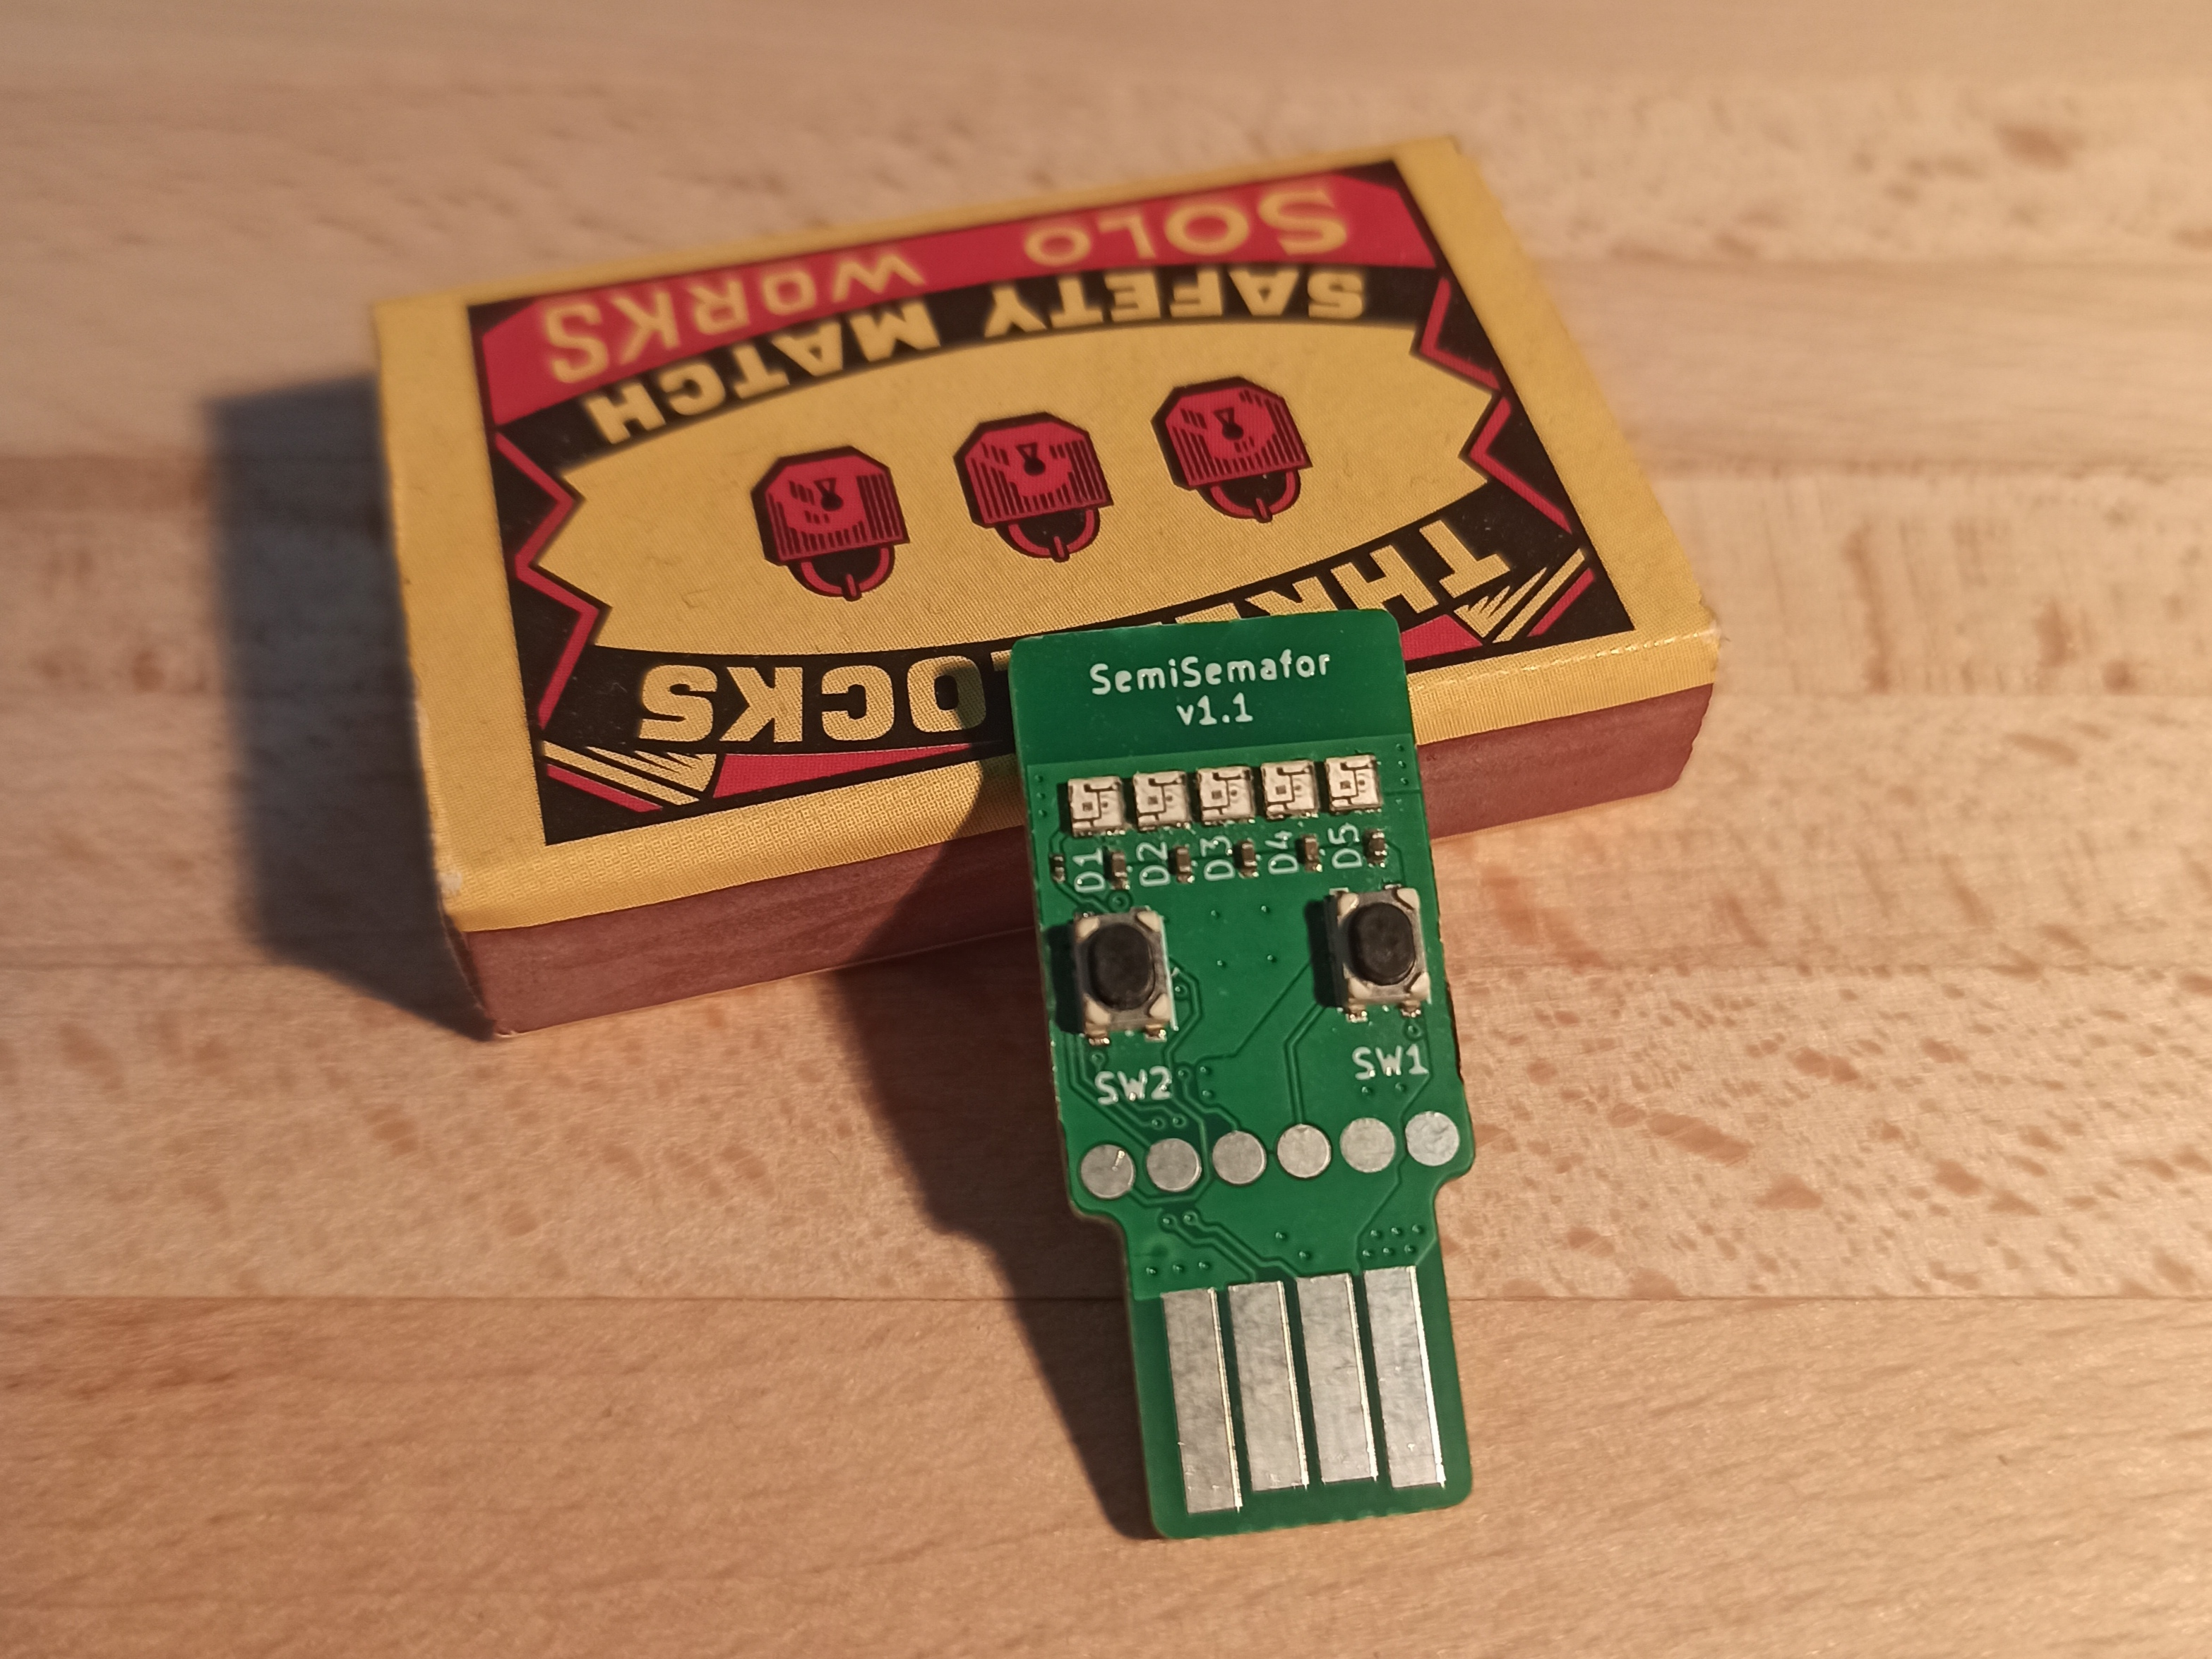
\includegraphics[width=0.8\textwidth]{text/TeoretickyUvod/AplikaceHernichZarizeni/img/1702085190411.jpg}
    \caption{Zařízení SemiSemafor}
    \label{fig:SemiSemafor}
\end{figure}

\subsection{Využití zařízení SemiSemafor}
SemiSemabor je využitelný například ve hře s názvem Duchové.



%%% Vložení souboru 'text/vysledky' s popisem vysledků práce
% (rozdělte na více souborů či kapitol, pokud je vhodné)
\chapter{Návrh zařízení}
\section{Úvodní specifikace}
Celé zařízení je rozděleno na základní jednotku a případné moduly které zajistí nové herní možnosti.
Například může jít o připojení úložného prostoru nebo zvukového modulu, který poskytne jak plnohodnotný zvukoví výstup tak vstup.

\subsection{uživatelské požadavky}
Jde o statické zařízení sloužící jako herní stanoviště.
Vyžaduje tedy mobilitu ale jen v rámci transportu na místo hry a spt, nikoliv v rámci samotné hry.

Zařízení bude mít dva světelné kruhy složené z inteligentních RGB LED.
Jeden radiální a druhý axiální na horní straně zařízení sloužící primárně jako odezva pro hráče na malou vzdálenost, např. při zadávání hesla.
Radiální kruh, také v horní části zařízení slouží naopak pro signalizace na delší vzdálenost, takový maják.

Uvnitř axiálního světelného kruhu se bude nacházet tzv. tlaková plocha.
Jedná se o ovládací prvek podobný dotykové ploše, s tím rozdílem že je schopen měřit i silu která na něj působí.

Aby bylo stanoviště reálně použitelné při hře musí celou hru vydržet na baterii.
Není ojedinělé aby měla outdoorová hra čtyři pět hodin bez přestávky.
Plus je nutná nějaká rezerva a čas na nastavování.
Pochopitelně je čas který zařízení zvládne běžet z baterie, silně závisí na činnosti, ale nebylo mi zrovna ideální, kdyby byla baterka, nějak výrazně omezující.
Výdrž na jedno nabití bych tedy chtěl směřovat alespoň na pět hodin.

Vzhledem k plánu připojovat moduly je nutné vyřešit jak se to budě dělat.
Bylo by ideální kdyby si mohl uživatel říct co bude hrát za hru a podle toho si sám připojil moduly které potřebuje.
Tomuto určitě nechceme bránit ale přímo to podporovat nese řadu problému jak ze strany konektoru a mechaniky, tak ze strany softwaru.
Konektor by totiž musel být ideálně beznástrojové rozpojitelný a opětovně spojitelný a přitom dostatečně pevný aby se zařízení mechanicky chovalo jako jeden celek.
Takový konektor je ale poměrně složité udělat tak aby byl spolehliví a tak jde v tuto chvíli spíš o hudbu budoucnosti.
Ze softwarového pohledu jde pak o problém z duvodu detekce konkrétních modulu a hlavně o otázku jak se chovat k modulum které jsou potenciálně záměnné.
Dejme tomu že máme modul klávesnici a modul dvířka.
Dvířka jsou původně primárně úložný prostor, díky detekci zavření je lze ale použít i jako velmi pohodlná tlačítka a v některých hrách se proto používají jen jako tlačítka.
Potenciální modul klávesnice je ovšem jen suma tlačítek.
Při vytváření konkrétní hry na míru modulum které herní návrhář má zrovna k dispozici je tento problém nepodstatný protože sám návrhář rozhodně co má jak být.
Ale ve chvíli kdy je ale o hru navrženou pro jinou kombinaci modulu nastává problém jak rozhodnout zda se dají dvířka použít místo klávesnice nebo ne.
Abychom se všem temto problémům, alespoň prozatím vyhnuli, rozhodli jsme že doplnění, či výměna modulu, pujde jen při servisním zásahu.

Některé hry vyžadují tak velké herní území že by na komunikaci mezi stanovišťmi už nestačila WiFi ani Bluetooth, které AHS jinak využívá ke komunikaci.  
Proto bude mít AHS možnost připojení k mobilní síti a tedy připojení k internetu.
Tím se za prvé rozšíří dosah AHS, všude kde je mobilní pokrytí a také přibude další metoda jak se stanovištěm komunikovat.
V rámci tohoto komunikačního modulu bude možné používat navíc i GNSS \footnote{Global Navigation Satellite System}.
Vzhledem k faktu že se přece jen nejedná o systém, který by využila většina her a zároveň je poměrně drahý došli jsme k rozhodnutí, mít jej jen jako doplnitelný modul.
Protože se jedná o modul který zprostředkovává komunikaci se světem je pravděpodobné že bude potřebovat převádět výrazně větší množství dat než běžný modul.
Primárně z tohoto důvodu je tento modul připojen na samostatném konektoru.
Potřebné antény budou už v základním zařízení ale samotný modul spadá do doplňkové výbavy.

V řadě případu je užitečné mít možnost zvuková zpětné vazby.
Ideální by bylo moci přehrávat libovolnou nahrávku, většinou ale stačí jednoduchý ton jako řekněme potvrzení na zadané heslo.
Možnost přehrávat plnohodnotnou nahrávku proto odsouváme jako možný doplňkový modul a v základní jednotce pro jednoduchost postačí piezoměnič. 


% \begin{itemize}
%     \item Dva LED kruhy jeden radiální na horní straně zařízení a jeden axiální v horní části zařízení
%     \item Tlaková plocha
%     \item Výdrž na baterii alespoň pět hodin aby bylo možné organizovat čtyřhodinovou hru s rezervou na nastavování atd.
%     \item Servisně snadné připojený komunikační/GPS modul uvnitř zařízení
%     \item Servisně snadné připojená dvířka a jiné moduly vně základního zařízení
%     \item Základní zvuková odezva
% \end{itemize}

\subsection{Struktura elektroniky základní jednotky}

Elektronika je rozdělena na tři samostatné PCB.
Jde o HlavníDeska na které je většina elektroniky, o~desku s~hlavním uživatelským rozhraním (LedDeska) a~o~obslužnou desku s~minimalistickým uživatelským rozhraním pro neherní obsluhu (MiniUI).

\subsubsection{LedDesku}
Jak název napovídá na LedDesce se nacházejí oba světelné kruhy, mimo to je zde i elektronika pro snímání tlakové plochy, tedy LDC1x14 \cite{LDC1614} a jeho snímací cívky.
Právě snímaní tlakové plochy je jeden z podstatných duvodu oddělení této desky od zbytku, zabere totiž docela dost prostoru.

\begin{itemize}
    \item Axiální LED kruh z 60ti RGB LED WS2812
    \item Zadní radiální LED kruh z 60ti RGB LED WS2812
    \item LDC1614 nebo LDC1314 se čtyřmi snímacími cívkami pro snímání tlakové plochy
    \item konektor na propojení s HlavníDeskou
\end{itemize}

\subsubsection{Mini UI}
Kvuli aktuální představě mechanické konstrukce není úplně dobře možné mít toto minimalistické uživatelské rozhraní na HlavníDeska.
Proto sme se rozhodli jej vyseparovat na samostatnou destičku, na které bude jen pár tlačítek a dvě signalizační LED.

\begin{itemize}
    \item RESET tlačítka
    \item BOOT tlačítka
    \item zapínací tlačítko
    \item dvě uživatelská tlačítka 
    \item dvě uživatelské ledky
\end{itemize}

\subsubsection{HlavníDeska}
Na HlavníDesce je většina systému základního zařízení.
Aby bylo možné určit chování celého zařízení je potřebný nějaký mikrokontroler.
Protože máme dlouholetým zkušenostem s mikrokontrolery ESP32, rozhodovali jsme jen mezi konkrétními verzemi z této rodiny.
% Dnes už tedy jen většina, mikrokontroleru této rodiny má integrovanou WiFi a Bluetooth periferii, kterou AHS určitě využije.
Aktuální plán na tvorbu vysoko-úrovňového návrhu konkrétních her je používat skriptovací jazyk JavaScript, považujeme za nevhodné provádět tento návrh na úrovní jazyka C/C++.
Abychom tohoto mohli dosáhnout, musíme provozovat nějaký interpreter JavaScriptu a z aktuálně dostupných možností, považujeme za nejideálnější Jaculus \cite{Jaculus}.
Jaculus dělá řadu věcí paralelně a je tím pádem pro jeho chod ideální mít více jader procesoru, což aktuálně znamená tři možnosti ESP32, ESP32S2 a ESP32S3.
ESP32S2 nemá Bluetooth, který bychom rádi měli k dispozici.
ESP32S3 je téměř jen vylepšená verze staršího ESP32, oproti tomu mu sice chybí pár možností, ty ale v AHS nepotřebujeme využívat a naopak se nám hodí vyšší výpočetní výkon, rychlejší paměť a více piny.
AHS tedy ovládá mikrokontroler ESP32S.




\begin{itemize}
    \item micro kontroler
    \item systém na dohodnutí PD
    \item bzučák (bez oscilátorové)
    \item Power manager
    \begin{itemize}
        \item připojení na dva paralelní LiIon články 18650
        \item hardwarová ochrana podvybití
        \item hardwarové řešení zapínání s ovládáním vyvedeným na MiniUI
        \item nabíječka
        \item step-up na 5V
        \item LDO na 3V3
        \item LDO na 1V8
    \end{itemize}
    \item Konektory
    \begin{itemize}
        \item LedDeska
        \item mini UI
        \item komunikační modul
        \item externí moduly
        \item USB-C (nabíjení a primární programování)
        \item případné zbylé piny
    \end{itemize}
\end{itemize}

\subsubsection{Popis jednotlivých bodů}
\paragraph{Micro kontroler}
všemu vládne je ESP32S3 \cite{ESP32S3-WR} až na to že něčemu ne.

\paragraph{Dohodnutí PD}
Komunikaci PD zajišťuje čip AP33772 \cite{AP33772} který je přes \(I2C\) připojený na ESP.

\paragraph{Bzučák}
Piezzo připojené mezi dva piny ESP aby bylo možné programově nastavit frekvenci a částečně i hlasitost.

\paragraph{Power manager}
\subparagraph{Zapínání}
Umožňuje uživateli zařízení zapínání tlačítkem.
Vypnutí je možné provést softwarově z ESP.

\subparagraph{Step-up na 5V}
Čip TPS61088 \cite{TPS61088} zajišťuje napájení světelným kruhům a externím modulům.
Je tedy schopen dodat proud pro oba světelné kruhy a moduloví konektor což znamená cca \(7\-[A]\).

\subparagraph{LDO na 3V3}
Zajišťuje napájení pro ESP32S3, LDC1x14 a PD sink AP33772 \cite{AP33772}.
Zároveň je z tohoto napětí odvozena větev 1.8V.
Proudově je tedy sto dodat cca \(1\-[A]\).

\subparagraph{LDO na 1V8}


\subparagraph{Nabíječka}
Nabíjení probíhá přes USB-C, nabíječka je proto schopna provozu z 5V.
Aby se ale zařízení dalo nabít rychleji je možno použít standard PowerDelivery s napětí až 21V.
Na nabíjení je proto použit chip BQ24179YBGR \cite{BQ24179}.

\subparagraph{Hw ochrana podvybití}
Kvuli ochraně baterie se zařízení vypne vypne při jejim vybití pod 2.8V.
Podle \cite{PanasonicLiOntReport} napětí na článek nesmí klesnout pod 2.3V. 
AHS k tomu volbou chipu BQ298012 \cite{BQ298012}, přidává rezervu 0.45V 



% ## Konektory
% ### USB-C
% D+ D- jsou napojeny přímo na ESP a CC piny jsou napojeny na AP33772(to přes I2C na ESP).

% ### Konektor komunikačního modulu
% Na konektor, je z ESP vyvedeno: 
% -   I2C
% -   celý UART
% -   FUL_CARD_POWER_OFF
% -   RESET
% -   WoWWAN (interrupt)

% a mimo ESP je na konektoru:
% -   napájení přímo z baterie
% -   SIM

% Pin-out M2 konektoru z https://files.waveshare.com/upload/0/02/SIM7600X-M2_Hardware_Design_V1.01.pdf
% ![](img/SIM7600G-H-M.2-PIN.png)

% ### Konektor na LedDesku

% <-1--13-> 5V

% <----14-> LED-DO

% <-15-27-> GND

% <----28-> 3V3

% <----29-> LDC-GND

% -----30-> LDC-INT

% <----31-> SDA

% <----32-- SCL


% Pull-upy na I2C a na LDC-INT mají 4.7kΩ.
% LDC-GND je na hlavní desce normální GND ale kvůli velkým proudum do ledek je v kabelu a na Led desce vedena odděleně.
% Konektorem na 5V proteče alespoň 5A.

% ### Moduloví konektor

% ---> USART-RX

% <--> 5V

% <--> GND

% <--- USART-TX

% <--> GND

% <--> 5V

% ---> INI

% Všechny moduly jsou připojeny na jeden RX pin AHS.
% Proto musí firmware AHS zajistit aby dva moduli nevysílali současně!
% Každý modul má TX připojen přes rezistor 180Ω jako ochranu.

% Interrupt na modulech se chová jako open-collector což je zajistit hardwarově.

% AHS zajišťuje odolnost proti rušení na všech vstupních vodičích pomocí 4.7kΩ pull-up a odolnost proti zkratu na datových výstupních vodičích pomocí 180Ω.
% Zároveň zajistí ESD ochranu všem vodičům co vedou z/do AHS.

% Konektor je zároveň sto dodat napájení 5V s proudem v součty 2A.

% Komunikace muže být vedena kabelem o délce až 25cm při komunikační rychlosti 5Mbps.
% *Při dalším prodlužování linky bude třeba vodiče RX a TX vlnově přizpůsobit a doplnit linku terminátory*



% ## mechanická část
% Základ AHS je mechanicky krátký válec s tlakovou plochou na horní ploše.
% Kolem tlakové plochu je umístěn axiální světelný kruh a v horní části válcové plochy je radiální světelný kruh.

% - Tělo minimálně v prototypu tisknuté
% - Vyzkoušet různé provedení kontaktní plochy
%     - Stejně jako na předchozí verzi FR4 ale tlustší aby se tolik nekroutila
%     - PCB s hliníkovým jádrem + zalití do epoxidu nebo jiné dostatečně průsvitné hmoty
% - Konektor externích modulu, USB-C a mini UI překrýt krytkou (ochrana před bordelem a náhodným mačkáním na tlačítka) 

% ![](img/dvirka.png)


%%% Vložení souboru 'text/zaver' se závěrem
\chapter*{Závěr}
\phantomsection
\addcontentsline{toc}{chapter}{Závěr}

Shrnutí studentské práce.


%%% Vložení souboru 'text/literatura' se seznamem zdrojů
% Pro sazbu seznamu literatury použijte jednu z následujících možností

%%%%%%%%%%%%%%%%%%%%%%%%%%%%%%%%%%%%%%%%%%%%%%%%%%%%%%%%%%%%%%%%%%%%%%%%%
%1) Seznam citací definovaný přímo pomocí prostředí literatura / thebibliography

% \begin{thebibliography}{99}
	
% \bibitem{sr72/2017}
% 	VYSOKÉ UČENÍ TECHNICKÉ V~BRNĚ.
% 	\emph{Směrnice č.\,72/2017, Úprava, odevzdávání a~zveřejňování závěrečných prací.}
% 	Online. Brno: VUT v~Brně, 2017.
% 	Úplné znění ke dni 11.\,4.\,2022.
% 	Dostupné z:\\
% 	{\small
% 	\url{https://www.vut.cz/uredni-deska/vnitrni-predpisy-a-dokumenty/smernice-c-72-2017-uprava-odevzdavani-a-zverejnovani-zaverecnych-praci-d161410}.}
% 	[cit.\ 2023-09-27].

% \bibitem{CSN_ISO_690-2022}
%     ÚŘAD PRO TECHNICKOU NORMALIZACI, METROLOGII A~STÁTNÍ ZKUŠEBNICTVÍ.
%     ČSN ISO 690:2022 (01 0197), \emph{Informace a dokumentace -- Pravidla pro bibliografické odkazy a~citace informačních zdrojů.}
%     Čtvrté vydání. Praha, 2022.

% \bibitem{CSN_ISO_7144-1997}
%     ÚŘAD PRO TECHNICKOU NORMALIZACI, METROLOGII A~STÁTNÍ ZKUŠEBNICTVÍ.
%     ČSN ISO 7144 (010161), \emph{Dokumentace -- Formální úprava disertací a~podobných dokumentů.}
% %    24 stran.
%     Praha, 1997.

% \bibitem{CSN_ISO_31-11}
%     ÚŘAD PRO TECHNICKOU NORMALIZACI, METROLOGII A~STÁTNÍ ZKUŠEBNICTVÍ.
%     ČSN ISO 31-11, \emph{Veličiny a~jednotky -- část 11: Matematické znaky a~značky používané ve fyzikálních vědách a~v~technice.}
%     Praha, 1999.

% \bibitem{Farkasova23:CSNISO6902022komentar}
% 	FARKAŠOVÁ, B. et al.
% 	\emph{Výklad normy ČSN ISO 690:2022 (01 0197) účinné od 1.\,12.\,2022}.
% 	 Online. První vydání. 2023.
% 	Dostupné~z:
% 	\url{https://www.citace.com/Vyklad-CSN-ISO-690-2022.pdf}.
% 	[cit.\,2023-09-27].

% \bibitem{pravidla}
%     \emph{Pravidla českého pravopisu}.
% 	1.\ vydání. Olomouc: FIN, 1998.\\
% 	\mbox{ISBN 80-86002-40-3}.

% \bibitem{Walter1999}
% 	WALTER, G.\,G. a SHEN, X.
% 	\emph{Wavelets and Other Orthogonal Systems}.
% 	2.\,vydání, Boca Raton: Chapman\,\&\,Hall/CRC, 2000.
% 	ISBN 1-58488-227-1

% \bibitem{Svacina1999IEEE}
% 	SVAČINA, J.
% 	Dispersion Characteristics of Multilayered Slotlines -- a Simple Approach.
% 	\emph{IEEE Transactions on Microwave Theory and Techniques}.
% 	1999, vol.\,47, no.\,9, s.\,1826--1829. ISSN 0018-9480.

% \bibitem{RajmicSysel2002}
%     RAJMIC, P. a SYSEL, P.
%     Wavelet Spectrum Thresholding Rules.
%     In: \emph{Proceedings of the International Conference Research in Telecommunication Technology}.
%     Žilina: Žilina University, 2002. s.\,60--63. ISBN 80-7100-991-1.

% \end{thebibliography}


%%%%%%%%%%%%%%%%%%%%%%%%%%%%%%%%%%%%%%%%%%%%%%%%%%%%%%%%%%%%%%%%%%%%%%%%%
%%2) Seznam citací pomocí BibTeXu
%% Při použití je nutné v TeXnicCenter ve výstupním profilu aktivovat spouštění BibTeXu po překladu.
%% Definice stylu seznamu
\bibliographystyle{unsrturl}
%% Pro českou sazbu lze použít styl czechiso.bst ze stránek
%% http://www.fit.vutbr.cz/~martinek/latex/czechiso.tar.gz
\bibliographystyle{czechiso}
%% Vložení souboru se seznamem citací
\bibliography{text/literatura.bib}
%
%% Následující příkaz je pouze pro ukázku sazby literatury při použití BibTeXu.
%% Způsobí citaci všech zdrojů v souboru literatura.bib, i když nejsou citovány v textu.
\nocite{*}

%%% Vložení souboru 'text/zkratky' se seznam použitých symbolů, veličin a zkratek
\cleardoublepage
\chapter*{\listofabbrevname}
\phantomsection
\addcontentsline{toc}{chapter}{\listofabbrevname}

\begin{acronym}[KolikMista]

	\acro{zkTemp}		% název
		[Šířka levého sloupce Seznamu symbolů a zkratek]								% zkratka
		{je určena šířkou parametru prostředí \texttt{acronym} (viz řádek~1 výpisu zdrojáku na~str.\,\pageref{lst:zkratky})}
											% rozvinutí zkratky

	\acro{AHS}
		{Automatické Herní Stanoviště}

	\acro{LDO}		% název/zkratka
		{Low-dropout regulator - regulátor napětí s nízkým úbytkem}
											% rozvinutí zkratky
	%%% bsymfvz
	\acro{FFC}						% název
		[\ensuremath{f_\textind{vz}}] % symbol
		{Flexible flat cable - plochý ohební kabel}					% popis
	%%% esymfvz

\end{acronym}


%%% Začátek příloh
\appendix

%%% Vysázení seznamu příloh
% (vynechejte, pokud máte dvě nebo méně příloh)
\listofappendices

%%% Vložení souboru 'text/prilohy' s přílohami
% Obvykle je přítomen alespoň popis co najdeme na přiloženém médiu
\chapter{Některé příkazy balíčku \texttt{thesis}}

\section{Příkazy pro sazbu veličin a jednotek}

\begin{table}[!h]
  \caption[Přehled příkazů]{Přehled příkazů pro matematické prostředí }
  \begin{center}
  	\small
	  \begin{tabular}{|c|c|c|c|}
	    \hline
	    Příkaz    						& Příklad 					& Zdroj příkladu  							& Význam  \\
	    \hline\hline
	    \verb|\textind{...}|	& $\beta_\textind{max}$ 	& \verb|$\beta_\textind{max}$|	& textový index \\
	    \hline
	    \verb|\const{...}| 		& $\const{U}_\textind{in}$ 				& \verb|$\const{U}_\textind{in}$|		& konstantní veličina \\
	    \hline
	    \verb|\var{...}| 		& $\var{u}_\textind{in}$ & \verb|$\var{u}_\textind{in}$| & proměnná veličina \\
	    \hline
	    \verb|\complex{...}| 	& $\complex{u}_\textind{in}$ & \verb|$\complex{u}_\textind{in}$| & komplexní veličina \\
	    \hline
	    \verb|\vect{...}| 		& $\vect{y}$ 						& \verb|$\vect{y}$| & vektor \\
	    \hline
	    \verb|\mat{...}| 	& $\mat{Z}$ 						& \verb|$\mat{Z}$| & matice \\
	    \hline
	    \verb|\unit{...}| 		& $\unit{kV}$ 						& \verb|$\unit{kV}$|\quad či\ \, \verb|\unit{kV}| & jednotka \\
	    \hline
	  \end{tabular}
  \end{center}
\end{table}



%\newpage
\section{Příkazy pro sazbu symbolů}

\begin{itemize}
  \item
    \verb|\E|, \verb|\eul| -- sazba Eulerova čísla: $\eul$,
  \item
    \verb|\J|, \verb|\jmag|, \verb|\I|, \verb|\imag| -- sazba imaginární jednotky: $\jmag$, $\imag$,
  \item
    \verb|\dif| -- sazba diferenciálu: $\dif$,
  \item
    \verb|\sinc| -- sazba funkce: $\sinc$,
  \item
    \verb|\mikro| -- sazba symbolu mikro stojatým písmem%
			\footnote{znak pochází z~balíčku \texttt{textcomp}}: $\mikro$,
	\item
		\verb|\uppi| -- sazba symbolu $\uppi$
			(stojaté řecké pí, na rozdíl od \verb|\pi|, což sází $\pi$).
\end{itemize}
%
Všechny symboly jsou určeny pro matematický mód, vyjma \verb|\mikro|, jenž je\\ použitelný rovněž v~textovém módu.
%$\upmikro$


\chapter{Druhá příloha}

\begin{figure}[!h]
  \begin{center}
    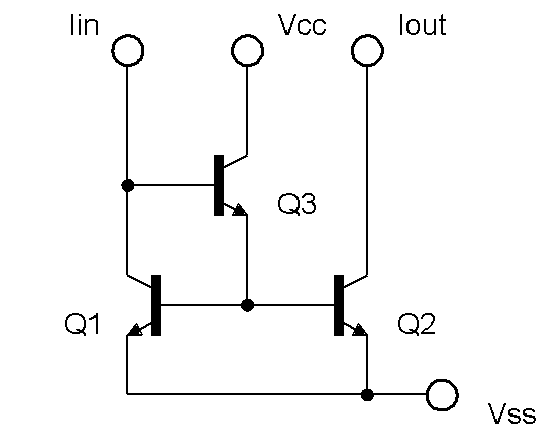
\includegraphics[scale=0.5]{obrazky/ZlepseneWilsonovoZrcadloNPN}
  \end{center}
  \caption[Alenčino zrcadlo]{Zlepšené Wilsonovo proudové zrcadlo.}
\end{figure}

Pro sazbu vektorových obrázků přímo v~\LaTeX{}u je možné doporučit balíček \href{https://www.ctan.org/pkg/pgf}{\texttt{TikZ}}.
Příklady sazby je možné najít na \href{http://www.texample.net/tikz/examples/}{\TeX{}ample}.
Pro vyzkoušení je možné použít programy QTikz nebo TikzEdt.




\chapter{Příklad sazby zdrojových kódů}

\section{Balíček \texttt{listings}}

Pro vysázení zdrojových souborů je možné použít balíček \href{https://www.ctan.org/pkg/listings}{\texttt{listings}}.
Balíček zavádí nové prostředí \texttt{lstlisting} pro sazbu zdrojových kódů, jako například:
%
\begin{lstlisting}[language={[LaTeX]TeX}]
\section{Balíček lstlistings}
Pro vysázení zdrojových souborů je možné použít
	balíček \href{https://www.ctan.org/pkg/listings}%
	{\texttt{listings}}.
Balíček zavádí nové prostředí \texttt{lstlisting} pro
	sazbu zdrojových kódů.
\end{lstlisting}
%
Podporuje množství programovacích jazyků.
Kód k~vysázení může být načítán přímo ze zdrojových souborů.
Umožňuje vkládat čísla řádků nebo vypisovat jen vybrané úseky kódu.
Např.:

\noindent
Zkratky jsou sázeny v~prostředí \texttt{acronym}:
\label{lst:zkratky}
\lstinputlisting[language={[LaTeX]TeX},nolol,numbers=left, firstnumber=6, firstline=6,lastline=6]{text/zkratky.tex}
%
Šířka textu volitelného parametru \verb|KolikMista| udává šířku prvního sloupce se zkratkami.
Proto by měla být zadávána nejdelší zkratka nebo symbol.
Příklad definice zkratky \acs{symfvz} je na výpisu \ref{lst:symfvz}.

\shorthandoff{-}
\lstinputlisting[language={[LaTeX]TeX},frame=single,caption={Ukázka sazby zkratek},label=lst:symfvz,numbers=left,linerange={bsymfvz-\%\%\%\ esymfvz},includerangemarker=false]{text/zkratky.tex}
\shorthandon{-}

\noindent
Ukončení seznamu je provedeno ukončením prostředí:
\lstinputlisting[language={[LaTeX]TeX},nolol,numbers=left,firstnumber=26,linerange=26]{text/zkratky.tex}

\vspace{\fill}

\noindent
{\bf Poznámka k~výpisům s~použitím volby jazyka \verb|czech| nebo \verb|slovak|:}\newline
Pokud Váš zdrojový kód obsahuje znak spojovníku \verb|-|, pak překlad může skončit chybou.
Ta je způsobená tím, že znak \verb|-| je v~českém nebo slovenském nastavení balíčku \verb|babel| tzv.\ aktivním znakem.
Přepněte znak \verb|-| na neaktivní příkazem \verb|\shorthandoff{-}| těsně před výpisem a hned za ním jej vraťte na aktivní příkazem \verb|\shorthandon{-}|.
Podobně jako to je ukázáno ve zdrojovém kódu šablony.


\clearpage

%\section{Výpis kódu prostředí Matlab}
Na výpisu \ref{lst:priklad.vypis.kodu.Matlab} naleznete příklad kódu pro Matlab, na výpisu \ref{lst:priklad.vypis.kodu.C} zase pro jazyk~C.

\lstnewenvironment{matlab}[1][]{%
\iflanguage{czech}{\shorthandoff{-}}{}%
\iflanguage{slovak}{\shorthandoff{-}}{}%
\lstset{language=Matlab,numbers=left,#1}%
}{%
\iflanguage{slovak}{\shorthandon{-}}{}%
\iflanguage{czech}{\shorthandon{-}}{}%
}

\begin{matlab}[frame=single,float=htbp,caption={Příklad Schur-Cohnova testu stability v~prostředí Matlab.},label=lst:priklad.vypis.kodu.Matlab,numberstyle=\scriptsize, numbersep=7pt]
%% Priklad testovani stability filtru

% koeficienty polynomu ve jmenovateli
a = [ 5, 11.2, 5.44, -0.384, -2.3552, -1.2288];
disp( 'Polynom:'); disp(poly2str( a, 'z'))

disp('Kontrola pomoci korenu polynomu:');
zx = roots( a);
if( all( abs( zx) < 1))
    disp('System je stabilni')
else
    disp('System je nestabilni nebo na mezi stability');
end

disp(' '); disp('Kontrola pomoci Schur-Cohn:');
ma = zeros( length(a)-1,length(a));
ma(1,:) = a/a(1);
for( k = 1:length(a)-2)
    aa = ma(k,1:end-k+1);
    bb = fliplr( aa);
    ma(k+1,1:end-k+1) = (aa-aa(end)*bb)/(1-aa(end)^2);
end

if( all( abs( diag( ma.'))))
    disp('System je stabilni')
else
    disp('System je nestabilni nebo na mezi stability');
end
\end{matlab}

\noindent
\begin{minipage}{\linewidth}


%\section{Výpis kódu jazyka C}

\begin{lstlisting}[frame=single,numbers=right,caption={Příklad implementace první kanonické formy v~jazyce C.},label=lst:priklad.vypis.kodu.C,basicstyle=\ttfamily\small, keywordstyle=\color{black}\bfseries\underbar,]
// první kanonická forma
short fxdf2t( short coef[][5], short sample)
{
	static int v1[SECTIONS] = {0,0},v2[SECTIONS] = {0,0};
	int x, y, accu;
	short k;

	x = sample;
	for( k = 0; k < SECTIONS; k++){
		accu = v1[k] >> 1;
		y = _sadd( accu, _smpy( coef[k][0], x));
		y = _sshl(y, 1) >> 16;

		accu = v2[k] >> 1;
		accu = _sadd( accu, _smpy( coef[k][1], x));
		accu = _sadd( accu, _smpy( coef[k][2], y));
		v1[k] = _sshl( accu, 1);

		accu = _smpy( coef[k][3], x);
		accu = _sadd( accu, _smpy( coef[k][4], y));
		v2[k] = _sshl( accu, 1);

		x = y;
	}
	return( y);
}
\end{lstlisting}
\end{minipage}







\chapter{Obsah elektronické přílohy}
Elektronická příloha je často nedílnou součástí semestrální nebo závěrečné práce.
Vkládá se do informačního systému VUT v~Brně ve vhodném formátu (ZIP, PDF\,\dots).

Nezapomeňte uvést, co čtenář v~této příloze najde.
Je vhodné okomentovat obsah každého adresáře, specifikovat, který soubor obsahuje důležitá nastavení, který soubor je určen ke spuštění, uvést nastavení kompilátoru atd.
Také je dobře napsat, v~jaké verzi software byl kód testován (např.\ Matlab 2018b).
Pokud bylo cílem práce vytvořit hardwarové zařízení,
musí elektronická příloha obsahovat veškeré podklady pro výrobu (např.\ soubory s~návrhem DPS v~Eagle).

Pokud je souborů hodně a jsou organizovány ve více složkách, je možné pro výpis adresářové struktury použít balíček \href{https://www.ctan.org/pkg/dirtree}{\texttt{dirtree}}.

\bigskip

{\small
%
\dirtree{%.
.1 /\DTcomment{kořenový adresář přiloženého archivu}.
.2 logo\DTcomment{loga školy a fakulty}.
.3 BUT\_abbreviation\_color\_PANTONE\_EN.pdf.
.3 BUT\_color\_PANTONE\_EN.pdf.
.3 FEEC\_abbreviation\_color\_PANTONE\_EN.pdf.
.3 FEKT\_zkratka\_barevne\_PANTONE\_CZ.pdf.
.3 UTKO\_color\_PANTONE\_CZ.pdf.
.3 UTKO\_color\_PANTONE\_EN.pdf.
.3 VUT\_barevne\_PANTONE\_CZ.pdf.
.3 VUT\_symbol\_barevne\_PANTONE\_CZ.pdf.
.3 VUT\_zkratka\_barevne\_PANTONE\_CZ.pdf.
.2 obrazky\DTcomment{ostatní obrázky}.
.3 soucastky.png.
.3 spoje.png.
.3 ZlepseneWilsonovoZrcadloNPN.png.
.3 ZlepseneWilsonovoZrcadloPNP.png.
.2 pdf\DTcomment{pdf stránky generované informačním systémem}.
.3 student-desky.pdf.
.3 student-titulka.pdf.
.3 student-zadani.pdf.
.2 text\DTcomment{zdrojové textové soubory}.
.3 literatura.tex.
.3 prilohy.tex.
.3 reseni.tex.
.3 uvod.tex.
.3 vysledky.tex.
.3 zaver.tex.
.3 zkratky.tex.
%.2 navod-sablona\_FEKT.pdf\DTcomment{návod na používání šablony}.
.2 sablona-obhaj.tex\DTcomment{hlavní soubor pro sazbu prezentace k~obhajobě}.
%.2 readme.txt\DTcomment{soubor s~popisem obsahu CD}.
.2 sablona-prace.tex\DTcomment{hlavní soubor pro sazbu kvalifikační práce}.
.2 thesis.sty\DTcomment{balíček pro sazbu kvalifikačních prací}.
}
}


\end{document}